\documentclass{article}
\usepackage[utf8]{inputenc}
\usepackage[english]{babel}
\usepackage{amsmath} % basic math
\usepackage{mathtools} % eg \coloneqq
\usepackage{amssymb} % include symbols such as R for the Reals

\usepackage{listings}
\setlength{\jot}{10pt} % increase spacing between equations
\usepackage{color}

 
\definecolor{codegreen}{rgb}{0,0.6,0}
\definecolor{codegray}{rgb}{0.5,0.5,0.5}
\definecolor{codepurple}{rgb}{0.58,0,0.82}
\definecolor{backcolour}{rgb}{0.95,0.95,0.92}
 
\lstdefinestyle{standard}{
    backgroundcolor=\color{backcolour},   
    commentstyle=\color{codegreen},
    keywordstyle=\color{magenta},
    numberstyle=\tiny\color{codegray},
    stringstyle=\color{codepurple},
    basicstyle=\footnotesize,
    breakatwhitespace=false,         
    breaklines=true,                 
    captionpos=b,                    
    keepspaces=true,                 
    numbers=left,                    
    numbersep=5pt,                  
    showspaces=false,                
    showstringspaces=false,
    showtabs=false,                  
    tabsize=2}
\lstset{style=standard}


\title{Conditional Multivariate Gaussian}
\author{Gabriel Dernbach}
\date{09.05.19}

\begin{document}

\maketitle

The conditional distribution of a multivariat normal distribution is key to the formulation of Gaussian Processes. In the following we will derive how the conditional can be stated.
\bigbreak
The multivariat normal distribution is given by
$$\mathcal{N}(\boldsymbol{x},\boldsymbol{\mu}, \mathbf{\Sigma})
= p(\mathbf{x}) = \frac{1}{\sqrt{(2 \pi)^{p} \operatorname{det}(\Sigma)}} \exp \left(-\frac{1}{2}(\mathbf{x}-\boldsymbol{\mu})^{\mathrm{T}} \mathbf{\Sigma}^{-1}(\mathbf{x}-\boldsymbol{\mu})\right)$$

In order to condition the multivariat gaussian onto one of it's components we remember that by
$$p(A|B) = \frac{p(A,B)}{p(B)}$$
the conditional distribution is found by dividing the joint distribution by the respective marignal distribution we which to condition on. Our aim therefore is to find a proper expression for the joint distribution from which the marginal and conditional probabilities immediately follow. 
\bigbreak
To distinguish between different components of the multivariate gaussian we choose a partitioning as follows
$$\mathbf{x}=\left[ \begin{array}{l}{\mathbf{x}_{1}} \\ {\mathbf{x}_{2}}\end{array}\right] \\ \mu=\left[ \begin{array}{c}{\mu_{1}} \\ {\mu_{2}}\end{array}\right] \quad \text { and } \quad {\mathbf{\Sigma}}=\left[ \begin{array}{cc}{\Sigma_{11}} & {\Sigma_{12}} \\ {\Sigma_{21}} & {\Sigma_{22}}\end{array}\right]$$
Where $\mathbf{x}$ is of dimension $n$ and $\mathbf{x_1}$,$\mathbf{x_2}$ are of dimension $p,q$ such that $n = p + q$. The marginal distributions of $\mathbf{x_1}$ and $\mathbf{x_2}$ are normal with $\mu_1$, $\mu_2$ and $\Sigma_1$, $\Sigma_2$ respectively.

By introducing the block notation we hope to find an untangled expression for the joint distribution in that it allows easy marginalization. The joint distribution is
\begin{align*}
	p(\mathbf{x})&=p\left(\mathbf{x}_{1}, \mathbf{x}_{2}\right) \\
		     &=\frac{1}{(2 \pi)^{n / 2}|\mathbf{\Sigma}|^{1 / 2}} \exp \left[-\frac{1}{2}(\mathbf{x}-\mu)^{T} \Sigma^{-1}(\mathbf{x}-\mu)\right] \\
		     &=\frac{1}{(2 \pi)^{n / 2}|\Sigma|^{1 / 2}} \exp \left[-\frac{1}{2} Q\left(\mathbf{x}_{1}, \mathbf{x}_{2}\right)\right]
\end{align*}

where $Q$ is the quadratic form which will take our primary attention from now on. The quadratic form after inserting the partitioning becomes

$$
\begin{aligned}
Q\left(\mathbf{x}_{1}, \mathbf{x}_{2}\right) &=(\mathbf{x}-\mu)^{T} \Sigma^{-1}(\mathbf{x}-\mu) \\
&=\left[\left(\mathbf{x}_{1}-\mu_{1}\right)^{T},\left(\mathbf{x}-\mu_{2}\right)^{T}\right] \left[ \begin{array}{cc}{\Sigma^{11}} & {\Sigma^{12}} \\ {\Sigma^{21}} & {\Sigma^{22}}\end{array}\right] \left[ \begin{array}{l}{\mathbf{x}_{1}-\mu_{1}} \\ {\mathbf{x}_{2}-\mu_{2}}\end{array}\right]\\
&=\left(\mathbf{x}_{1}-\mu_{1}\right)^{T} \Sigma^{11}\left(\mathbf{x}_{1}-\mu_{1}\right)\\
&\quad+2\left(\mathbf{x}_{1}-\mu_{1}\right)^{T} \Sigma^{12}\left(\mathbf{x}_{2}-\mu_{2}\right)\\
&\quad+\left(\mathbf{x}_{2}-\mu_{2}\right)^{T} \Sigma^{22}\left(\mathbf{x}_{2}-\mu_{2}\right) 
\end{aligned}
$$

where we introduced the following notation for the partitioned inverse
$$
\Sigma^{-1}=\left[ \begin{array}{cc}{\Sigma_{11}} & {\Sigma_{12}} \\ {\Sigma_{21}} & {\Sigma_{22}}\end{array}\right]^{-1}=\left[ \begin{array}{cc}{\Sigma^{11}} & {\Sigma^{12}} \\ {\Sigma^{21}} & {\Sigma^{22}}\end{array}\right]
$$

As we have assumed a block representation of the inverted block covariance matrix, let us now examine how the original blocks behave under inversion. In this rather general examination of a symmetric block matrix under inversion we will substitute A for the matrix and B for it's inverse in order to facilitate readability.

$$
\begin{aligned} I_{n} &=A A^{-1}=A B=\left[ \begin{array}{cc}{A_{11}} & {A_{12}} \\ {A_{12}^{T}} & {A_{22}}\end{array}\right] \left[ \begin{array}{cc}{B_{11}} & {B_{12}} \\ {B_{12}^{T}} & {B_{22}}\end{array}\right] \\ &=\left[ \begin{array}{cc}{A_{11} B_{11}+A_{12} B_{12}^{T}} & {A_{11} B_{12}+A_{12} B_{22}} \\ {A_{12}^{T} B_{11}+A_{22} B_{12}^{T}} & {A_{12} B_{12}+A_{22} B_{22}}\end{array}\right]=\left[ \begin{array}{cc}{I_{p}} & {0} \\ {0} & {I_{q}}\end{array}\right] \end{aligned}
$$

By comparison of coefficients we can find expressions for the entries $B_{11},B_{12},B_{21},B_{22}$ of our inverse symmetric block matrix, which are
\begin{alignat*}{3}
A_{11} B_{11}+A_{12} B_{12}^{T}=I_{p} & \quad \implies \quad &&  B_{11}=A_{11}^{-1}-A_{11}^{-1} A_{12} B_{12}^{T} \\
A_{11} B_{12}+A_{12} B_{22}=0 & \quad \implies \quad && B_{12}=-A_{11}^{-1} A_{12} B_{22} \\
A_{12}^{T} B_{11}+A_{22} B_{12}^{T}=0 & \quad \implies \quad && B_{22}=-A_{22}^{-1} A_{12}^{T} B_{11} \\
A_{12}^{T} B_{12}+A_{22} B_{22}=I_{q} & \quad \implies \quad && B_{22}=A_{22}^{-1}-A_{22}^{-1} A_{12}^{T} B_{12}
\end{alignat*}

We continue our pursuit of expressions of $B$ that are purely stated in terms of $A$. 
First we can introduce $B_{12}^\top$ into the equation of $B_{11}$ to get
\begin{align*}
	B_{11}=& A_{11}^{-1}+A_{11}^{-1} A_{12} A_{22}^{-1} A_{12}^{T} B_{11} \\ 
	A_{11}^{-1} =& \left(I-A_{11}^{-1} A_{12} A_{22}^{-1} A_{12}^{T}\right) B_{11}\\
	I_{p} =& \left(A_{11}-A_{12} A_{22}^{-1} A_{12}^{T}\right) B_{11} \\
	B_{11}=& \left(A_{11}-A_{12} A_{22}^{-1} A_{12}^{T}\right)^{-1}
\end{align*}

Simillarly we can substitute $B_{12}$ into the equation of $B_{22}$, as well as using these intermediat results to recover the remaining block matrices $B_{12}$ and $B_{12}^\top$
\begin{align*}
B_{12}=&-A_{11}^{-1} A_{12}\left(A_{22}-A_{12}^{T} A_{11}^{-1} A_{12}^{-1}\right) \\
B_{12}^{T}=&-A_{22}^{-1} A_{12}^{T}\left(A_{11}-A_{12} A_{22}^{-1} A_{12}^{T}\right)^{-1} \\
B_{22}=&\left(A_{22}-A_{12}^{T} A_{11}^{-1} A_{12}\right)^{-1} 
\end{align*}

After this excursion to the inverse of block matrices we can substitute	back to the original notation of $\Sigma$ to see that
\begin{align*}
\Sigma^{11}&=\left(\Sigma_{11}-\Sigma_{12} \Sigma_{22}^{-1} \Sigma_{12}^{T}\right)^{-1} \\
\Sigma^{22}&=\left(\Sigma_{22}-\Sigma_{12}^{T} \Sigma_{11}^{-1} \Sigma_{12}\right)^{-1} \\
\Sigma^{12}&=-\Sigma_{11}^{-1} \Sigma_{12}\left(\Sigma_{22}-\Sigma_{12}^{T} \Sigma_{11}^{-1} \Sigma_{12}\right)^{-1}=\left(\Sigma^{21}\right)^{T}
\end{align*}

As we now have a way to translate a block covariance matrix to it's inverse block matrix we may find an expression for $Q((\mathbf{x_1},\mathbf{x_2}))$ in terms of the covariance matrix itself. Before substituting our current results into Q however, we can increase flexibility by splitting the product of component $\Sigma^{11}$ by the Sherman–Morrison–Woodbury formula into a sum. This will later turn out beneficial in cancelling related terms.
\bigbreak

The Woodburry matrix identity can be found by comparison of the inverse of two slightly differing decompositions of one matrix. A decomposition that is particularly nice to invert is the LDU decomposition, as the triangular parts will only change their sign \footnote{as can directly be shown by an ordinary gauss-jordan elimination.} and the inverse of the diagonal is found by elementwise inversion. We will therefore consider a block matrix $M$ of the form 


$$\left[ \begin{array}{ll}{A} & {U} \\ {V} & {C}\end{array}\right]$$
The parts of the decomposition can be found by successively multiplying matrices to $M$ such that it's offdiagonal elements are set to zero.

We start with an identity matrix which we try to alter in a way such that it will set the entry below A to zero. Next we note that the entry at $V$ after the multiplication with the identiy would be the consequence of $0 * A + 1 * V$. It is straight forward to set this equation to zero by finding a coefficient at the $0$ position of the identity matrix that cancels $V$. Such is $-VA^{-1} A + 1 V$. 
Therefore our first elimination results in
$$\left[ \begin{array}{cc}{I} & {0} \\ {-V A^{-1}} & {I}\end{array}\right] \left[ \begin{array}{cc}{A} & {U} \\ {V} & {C}\end{array}\right]=\left[ \begin{array}{cc}{A} & {U} \\ {0} & {C-V A^{-1} U}\end{array}\right]$$
Similarly the entry above C can be eliminated by
$$\left[ \begin{array}{cc}{A} & {U} \\ {V} & {C}\end{array}\right] \left[ \begin{array}{cc}{I} & {-A^{-1} U} \\ {0} & {I}\end{array}\right]=\left[ \begin{array}{cc}{A} & {0} \\ {V} & {C-V A^{-1} U}\end{array}\right]$$
Combining the two multiplications already yields the desired diagonal
$$\left[ \begin{array}{cc}{I} & {0} \\ {-V A^{-1}} & {I}\end{array}\right] \left[ \begin{array}{cc}{A} & {U} \\ {V} & {C}\end{array}\right] \left[ \begin{array}{cc}{I} & {-A^{-1} U} \\ {0} & {I}\end{array}\right]=\left[ \begin{array}{cc}{A} & {0} \\ {0} & {C-V A^{-1} U}\end{array}\right]$$
Moving to the right side yields the LDU decomposition of $M$
$$\left[ \begin{array}{ll}{A} & {U} \\ {V} & {C}\end{array}\right]=\left[ \begin{array}{cc}{I} & {0} \\ {V A^{-1}} & {I}\end{array}\right] \left[ \begin{array}{cc}{A} & {0} \\ {0} & {C-V A^{-1} U}\end{array}\right] \left[ \begin{array}{cc}{I} & {A^{-1} U} \\ {0} & {I}\end{array}\right]$$
Inverting both sides we see at the right a decomposition of the total inverse into it's block components.
\begin{align*}
	\left[ \begin{array}{cc}{A} & {U} \\ {V} & {C}\end{array}\right]^{-1}&=\left[ \begin{array}{cc}{I} & {A^{-1} U} \\ {0} & {I}\end{array}\right]^{-1} \left[ \begin{array}{cc}{A} & {0} \\ {0} & {C-V A^{-1} U}\end{array}\right]^{-1} \left[ \begin{array}{cc}{I} & {0} \\ {V A^{-1}} & {I}\end{array}\right]^{-1}\\
&=\left[ \begin{array}{cc}{I} & {-A^{-1} U} \\ {0} & {I}\end{array}\right] \left[ \begin{array}{cc}{A^{-1}} & {0} \\ {0} & {\left(C-V A^{-1} U\right)^{-1}}\end{array}\right] \left[ \begin{array}{cc}{I} & {0} \\ {-V A^{-1}} & {I}\end{array}\right]\\
&=\left[ \begin{array}{cc}{A^{-1}+A^{-1} U\left(C-V A^{-1} U\right)^{-1} V A^{-1}} & {-A^{-1} U\left(C-V A^{-1} U\right)^{-1}} \\ {-\left(C-V A^{-1} U\right)^{-1} V A^{-1}} & {\left(C-V A^{-1} U\right)^{-1}}\end{array}\right]
\end{align*}
\bigbreak
Now as a slightly differing approach, we could have equally likely chosen to first set the value above $C$ to zero. The latter approach results in
\begin{align*}
\left[ \begin{array}{cc}{A} & {U} \\ {V} & {C}\end{array}\right]=\left[ \begin{array}{cc}{I} & {U C^{-1}} \\ {0} & {I}\end{array}\right] \left[ \begin{array}{cc}{A-U C^{-1} V} & {0} \\ {0} & {C}\end{array}\right] \left[ \begin{array}{cc}{I} & {0} \\ {C^{-1} V} & {I}\end{array}\right]
\end{align*}
Inversion of both sides yields
\begin{align*}
\left[ \begin{array}{cc}{A} & {U} \\ {V} & {C}\end{array}\right]^{-1}&=\left[ \begin{array}{cc}{I} & {0} \\ {C^{-1} V} & {I}\end{array}\right]^{-1} \left[ \begin{array}{cc}{A-U C^{-1} V} & {0} \\ {0} & {C}\end{array}\right]^{-1} \left[ \begin{array}{cc}{I} & {U C^{-1}} \\ {0} & {I}\end{array}\right]^{-1} \\
&=\left[ \begin{array}{cc}{I} & {0} \\ {-C^{-1} V} & {I}\end{array}\right] \left[ \begin{array}{cc}{\left(A-U C^{-1} V\right)^{-1}} & {0} \\ {0} & {C^{-1}}\end{array}\right] \left[ \begin{array}{cc}{I} & {-U C^{-1}} \\ {0} & {I}\end{array}\right] \\
&=\left[ \begin{array}{cc}{\left(A-U C^{-1} V\right)^{-1}} & {-\left(A-U C^{-1} V\right)^{-1} U C^{-1}} \\ {-C^{-1} V\left(A-U C^{-1} V\right)^{-1}} & {C^{-1} V\left(A-U C^{-1} V\right)^{-1} U C^{-1}+C^{-1}}\end{array}\right]
\end{align*}

Inspecting the elements of the two approaches we note a discovery of different ways to write an equally valid block of the inverse, that is we found a matrix identity. Most notably is the identitiy given by the respective elements in the first row and column. This identity is commonly referred to as the Woodburry matrix identity, or matrix inversion lemma
$$\left(A-U C^{-1} V\right)^{-1}=A^{-1}+A^{-1} U\left(C-V A^{-1} U\right)^{-1} V A^{-1}$$

A direct proof of validity of our equality can be found by the fact that the following product evaluates to the identity matrix as expected
$$(A+U C V)\left[A^{-1}-A^{-1} U\left(C^{-1}+V A^{-1} U\right)^{-1} V A^{-1}\right]$$


We now can rewrite $\Sigma^{11}$ as it takes the exact from of the left hand side of the Woodburry Matrix Identity and thereby untangle it's product into a sum.

\bigbreak
We summarize the block inverses
\begin{align*}
\Sigma^{11}&=\left(\Sigma_{11}-\Sigma_{12} \Sigma_{22}^{-1} \Sigma_{12}^{T}\right)^{-1} \\
&=\Sigma_{11}^{-1}+\Sigma_{11}^{-1} \Sigma_{12}\left(\Sigma_{22}-A_{12}^{T} \Sigma_{11}^{-1} \Sigma_{12}\right)^{-1} \Sigma_{12}^{T} \Sigma_{11}^{-1} \\
\Sigma^{22}&=\left(\Sigma_{22}-\Sigma_{12}^{T} \Sigma_{11}^{-1} \Sigma_{12}\right)^{-1} \\
&=\Sigma_{22}^{-1}+\Sigma_{22}^{-1} \Sigma_{12}^{T}\left(\Sigma_{11}-\Sigma_{12} \Sigma_{22}^{-1} \Sigma_{12}^{T}\right)^{-1} \Sigma_{12} \Sigma_{22}^{-1} \\
\Sigma^{12}&=-\Sigma_{11}^{-1} \Sigma_{12}\left(\Sigma_{22}-\Sigma_{12}^{T} \Sigma_{11}^{-1} \Sigma_{12}\right)^{-1}=\left(\Sigma^{21}\right)^{T}
\end{align*}
We get back to the quadratic $Q(\mathbf{x_1},\mathbf{x_2})$ and substitute the second equation of $\Sigma^{11}$, the first equation of $\Sigma_{22}$ and $\Sigma_{12}$ 
\begin{align*}
Q\left(\mathbf{x}_{1}, \mathbf{x}_{2}\right)&=\left(\mathbf{x}_{1}-\mu_{1}\right)^{T} \Sigma^{11}\left(\mathbf{x}_{1}-\mu_{1}\right) \\
&\quad+2\left(\mathbf{x}_{1}-\mu_{1}\right)^{T} \Sigma^{12}\left(\mathbf{x}_{2}-\mu_{2}\right) \\
&\quad+\left(\mathbf{x}_{2}-\mu_{2}\right)^{T} \Sigma^{22}\left(\mathbf{x}_{2}-\mu_{2}\right) \\
Q\left(\mathbf{x}_{1}, \mathbf{x}_{2}\right)&=\left(\mathbf{x}_{1}-\mu_{1}\right)^{T}\left[\Sigma_{11}^{-1}+\Sigma_{11}^{-1} \Sigma_{12}\left(\Sigma_{22}-\Sigma_{12}^{T} \Sigma_{11}^{-1} \Sigma_{12}\right)^{-1} \Sigma_{12}^{T} \Sigma_{11}^{-1}\right]\left(\mathbf{x}_{1}-\mu_{1}\right) \\
&\quad -2\left(\mathbf{x}_{1}-\mu_{1}\right)^{T}\left[\Sigma_{11}^{-1} \Sigma_{12}\left(\Sigma_{22}-\Sigma_{12}^{T} \Sigma_{11}^{-1} \Sigma_{12}\right)^{-1}\right]\left(\mathbf{x}_{2}-\mu_{2}\right) \\
&\quad +\left(\mathbf{x}_{2}-\mu_{2}\right)^{T}\left[\left(\Sigma_{22}-\Sigma_{12}^{T} \Sigma_{11}^{-1} \Sigma_{12}\right)^{-1}\right]\left(\mathbf{x}_{2}-\mu_{2}\right)
\end{align*}
And expand the product in the first term
\begin{align*}
Q\left(\mathbf{x}_{1}, \mathbf{x}_{2}\right) &= \left(\mathbf{x}_{1}-\mu_{1}\right)^{T} \Sigma_{11}^{-1}\left(\mathbf{x}_{1}-\mu_{1}\right) \\ 
&\quad+\left(\mathbf{x}_{1}-\mu_{1}\right)^{T}\left[\Sigma_{11}^{-1} \Sigma_{12}\left(\Sigma_{22}-\Sigma_{12}^{T} \Sigma_{11}^{-1} \Sigma_{12}\right)^{-1} \Sigma_{12}^{T} \Sigma_{11}^{-1}\right]\left(\mathbf{x}_{1}-\mu_{1}\right) \\
&\quad -2\left(\mathbf{x}_{1}-\mu_{1}\right)^{T}\left[\Sigma_{11}^{-1} \Sigma_{12}\left(\Sigma_{22}-\Sigma_{12}^{T} \Sigma_{11}^{-1} \Sigma_{12}\right)^{-1}\right]\left(\mathbf{x}_{2}-\mu_{2}\right) \\
&\quad +\left(\mathbf{x}_{2}-\mu_{2}\right)^{T}\left[\left(\Sigma_{22}-\Sigma_{12}^{T} \Sigma_{11}^{-1} \Sigma_{12}\right)^{-1}\right]\left(\mathbf{x}_{2}-\mu_{2}\right)
\end{align*}
The second part resembles a quadratic form already that we only need to factorize. To see more clearly we define it's factors to be
\begin{align*}
u &\coloneqq \left(\mathbf{x}_{1}-\mu_{1}\right)^{T}\Sigma_{11}^{-1} \Sigma_{12}\\
v &\coloneqq \left(\mathrm{x}_{2}-\mu_{2}\right) \\
A &\coloneqq \Sigma_{22}-\Sigma_{12}^{T} \Sigma_{11}^{-1} \Sigma_{12} )^{-1}
\end{align*}
Which allows the standart factorization as
\begin{align*}
&u^{T} A u-2 u^{T} A v+v^{T} A v \\
=& u^{T} A u-u^{T} A v-u^{T} A v+v^{T} A v \\
=& u^{T} A(u-v)-(u-v)^{T} A v \\
=& u^{T} A(u-v)-v^{T} A(u-v) \\
=& (u-v)^{T} A(u-v) \\
=&(v-u)^{T} A(v-u)
\end{align*}

Introducing the factorization in $Q(\mathbf{x_1},\mathbf{x_1})$ yields
{\small
\begin{align*}
Q(\mathbf{x_1},\mathbf{x_2}) &= \left(\mathbf{x}_{1}-\mu_{1}\right)^{T} \Sigma_{11}^{-1}\left(\mathbf{x}_{1}-\mu_{1}\right) \\
&\quad + \left[\left(\mathbf{x}_{2}-\mu_{2}\right)-\Sigma_{12}^{T} \Sigma_{11}^{-1}\left(\mathbf{x}_{1}-\mu_{1}\right)\right]^{T} \\
&\quad \quad \quad \left(\Sigma_{22}-\Sigma_{12}^{T} \Sigma_{11}^{-1} \Sigma_{12}\right)^{-1}\left[\left(\mathbf{x}_{2}-\mu_{2}\right)-\Sigma_{12}^{T} \Sigma_{11}^{-1}\left(\mathbf{x}_{1}-\mu_{1}\right)\right]
\end{align*}
}

As it turns out, the quadratic is itself the sum of two quadratics again. Taking the sum out of the exponential, we can already anticipate the result of a product of gaussians. Whereas the first one has straight forward expected value of $\mu_1$ and covariance $\Sigma_{11}^{-1}$, we introduce a short hand for those parameters in the second as
\begin{align*}
b &\coloneqq \mu_{2}+\Sigma_{12}^{T} \Sigma_{11}^{-1}\left(\mathbf{x}_{1}-\mu_{1}\right)
  & A &\coloneqq \Sigma_{22}-\Sigma_{12}^{T} \Sigma_{11}^{-1} \Sigma_{12}
\end{align*}

At this point the joint distribution has become
\begin{align*}
p(\mathbf{x})&=p\left(\mathbf{x}_{1}, \mathbf{x}_{2}\right)=\frac{1}{(2 \pi)^{n / 2}|\Sigma|^{1 / 2}} \exp \left[-\frac{1}{2} Q\left(\mathbf{x}_{1}, \mathbf{x}_{2}\right)\right] \\
&= \frac{1}{(2 \pi)^{n / 2}|\Sigma|^{1 / 2}}\exp \left[-\frac{1}{2}\left(\mathbf{x}_{1}-\mu_{1}\right)^{T} \Sigma_{11}^{-1}\left(\mathbf{x}_{1}-\mu_{1}\right)\right] \exp \left[-\frac{1}{2}\left(\mathbf{x}_{2}-b\right)^{T} A^{-1}\left(\mathbf{x}_{2}-b\right)\right]
\end{align*}
Lastly we need to split the normalization into the respective blocks. First we note that the determinant of a product is the product of the determinants.
\begin{align*}
|A B|=|A||B|
\end{align*}
Together with the fact that
\begin{align*}
\left| \begin{array}{cc}{B} & {0} \\ {C} & {D}\end{array}\right|=\left| \begin{array}{cc}{B} & {C} \\ {0} & {D}\end{array}\right|=|B||D|
\end{align*}
We again turn to a triangular decomposition, this time however without the diagonal, which for a 2 by 2 matrix is
\begin{align*}
A=\left[ \begin{array}{ll}{A_{11}} & {A_{12}} \\ {A_{21}} & {A_{22}}\end{array}\right]=\left[ \begin{array}{cc}{A_{11}} & {0} \\ {A_{12}^{T}} & {I}\end{array}\right] \left[ \begin{array}{cc}{I} & {A_{11}^{-1} A_{12}} \\ {0} & {A_{22}-A_{12}^{T} A_{11}^{-1} A_{12}}\end{array}\right]
\end{align*}
Combinig the three observations gives the decomposition we need
\begin{align*}
|A|=\left| \left[ \begin{array}{cc}{A_{11}} & {A_{12}} \\ {A_{21}} & {A_{22}}\end{array}\right]\right| = \left|A_{11} \right| \left| A_{22}-A_{12}^{T} A_{11}^{-1} A_{12}\right|
\end{align*}
We therefore separate the determinant of the covariance matrix by
\begin{align*}
|\Sigma|=\left| \left[ \begin{array}{cc}{\Sigma_{11}} & {\Sigma_{12}} \\ {\Sigma_{21}} & {\Sigma_{22}}\end{array}\right]\right|=| \Sigma_{22}| | \Sigma_{11}-\Sigma_{12} \Sigma_{22}^{-1} \Sigma_{12}^{T}|=| \Sigma_{11} \| \Sigma_{22}-\Sigma_{12}^{T} \Sigma_{11}^{-1} \Sigma_{12} |	
\end{align*}
And see that the joint probability is indeed the product of two gaussians
\begin{align*}
p\left(\mathbf{x}_{1}, \mathbf{x}_{2}\right)&= \frac{1}{(2 \pi)^{p / 2}\left|\Sigma_{11}\right|^{1 / 2}} \exp \left[-\frac{1}{2}\left(\mathrm{x}_{1}-\mu_{1}\right)^{T} \Sigma_{11}^{-1}\left(\mathrm{x}_{1}-\mu_{1}\right)\right] \\
& \quad\quad \frac{1}{(2 \pi)^{\mathrm{q} / 2}|A|^{1 / 2}} \exp \left[-\frac{1}{2}\left(\mathrm{x}_{2}-b\right)^{T} A^{-1}\left(\mathrm{x}_{2}-b\right)\right] \\
&=\quad \mathcal{N}\left(\mathbf{x}_{1}, \mu_{1}, \Sigma_{11}\right) \mathcal{N}\left(\mathbf{x}_{2}, b, A\right)
\end{align*}

\bigbreak
The marginal distribution over $x_1$ is
\begin{align*}
p_{1}\left(\mathbf{x}_{1}\right)=\int p\left(\mathbf{x}_{1}, \mathbf{x}_{2}\right) d \mathbf{x}_{2}=\frac{1}{(2 \pi)^{p / 2}\left|\Sigma_{11}\right|^{1 / 2}} \exp \left[-\frac{1}{2}\left(\mathbf{x}_{1}-\mu_{1}\right)^{T} \Sigma_{11}^{-1}\left(\mathbf{x}_{1}-\mu_{1}\right)\right]
\end{align*}
As $p(x_2)$ is normalized and therefore integrates to 1. Altough we find a dependence on $x_1$ in the second gaussian, it is only in the mean vector $b$ that shifts the gaussian but lets its integral stay unchanged of course. 

Finally by dividing the joint by the marginal we arrive at the conditional distribution
\begin{align*}
p_{2|1}\left(\mathbf{x}_{2} | \mathbf{x}_{1}\right)=\frac{p\left(\mathbf{x}_{1}, \mathbf{x}_{2}\right)}{p\left(\mathbf{x}_{1}\right)}=\frac{1}{(2 \pi)^{q / 2}|A|^{1 / 2}} \exp \left[-\frac{1}{2}\left(\mathbf{x}_{2}-b\right)^{T} A^{-1}\left(\mathbf{x}_{2}-b\right)\right]
\end{align*}
with
\begin{align*}
b&=\mu_{2}+\Sigma_{12}^{T} \Sigma_{11}^{-1}\left(\mathbf{x}_{1}-\mu_{1}\right) \\
A&=\Sigma_{22}-\Sigma_{12}^{T} \Sigma_{11}^{-1} \Sigma_{12}
\end{align*}

\newpage

For a gaussian process regression we assume $\mu_1 = \mu_2 = 0$. An example of such a regression is given in matlab and python. We denote $x1,y1$ as the training data and $x2,y2$ as the predictions.


\begin{lstlisting}[language=Matlab, caption=matlab implementation of a gaussian process]
% specify distribution
x1 = [-1, -0.9, -0.4, -0.25, 0.5, 1];
y1 = [0, -1, 2, 0.5, 2, 0];
x2 = linspace(-1,1,1000);

% estimate posterior
[y2,sigma2] = gaussian_process(x1,y1,x2,width,lambda);


function [y2,sigma2] = gaussian_process(x1,y1,x2,width,lambda)
    k11 = kernel(x1,x1,width,lambda); % auto covariance of x1
    k12 = kernel(x2,x1,width,lambda); % cross covariance x1 to x2
    k22 = kernel(x2,x2,width,lambda); % auto covariance of x2
    
    y2 = k12' / k11 * y1'; % posterior mean prediction
    sigma2 = k22 - k12' / k11 * k12; % posterior variance prediction
end

function kab = kernel(a,b,width,lambda) % gaussain kernel
    kab = exp(-(a-b').^2 ./ (2*width^2)); % exponential pairwise
    kab = kab + eye(size(kab)) .* lambda; % regularization
end
\end{lstlisting}

\begin{lstlisting}[language=Matlab, caption=code to create the plots in fig. 1 and 2]
figure()
plot(x1,y1,'o','MarkerSize',7)
hold('on')
plot(x2,y2,'Color',[0, 0.4470, 0.7410],'Linewidth',3)
std2 = 1.96.*sqrt(diag(sigma2)); % extract 95 percent quantile
plot(x2,y2+std2,'Color',[0.8500, 0.3250, 0.0980],'Linewidth',0.05)
plot(x2,y2-std2,'color',[0.8500, 0.3250, 0.0980],'Linewidth',0.05)
title('mean prediction and 95 percentile')
legend('prior','mean prediction',' 95 percentile')

figure()
for i = 1:8
    plot(x2,mvnrnd(y2,sigma2)); hold('on')
    title('8 realizations of the distribution')
end
\end{lstlisting}



\begin{figure}
\centering
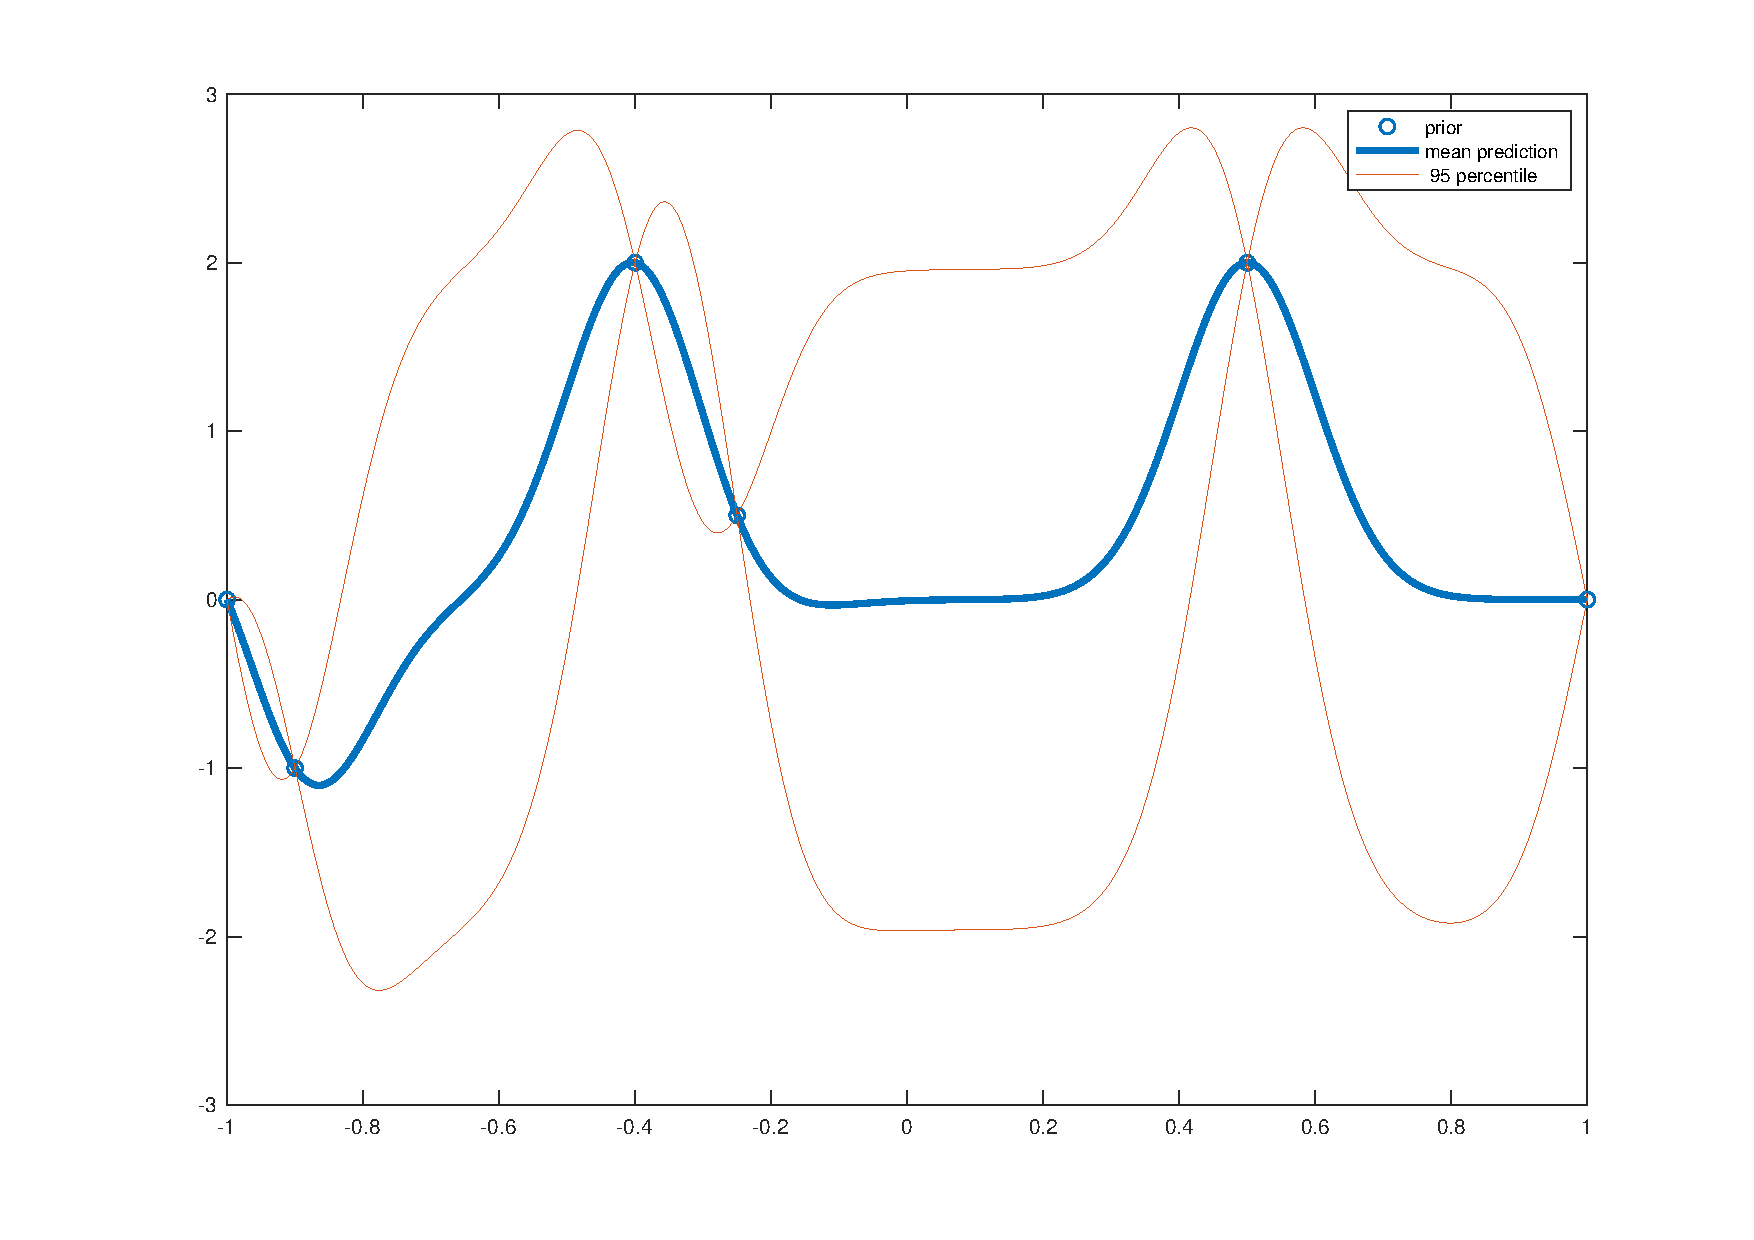
\includegraphics[width=.9\linewidth]{fig/mean.pdf}
\caption{A gaussian process that fulfills the specified points and has increased variance where the process is less determined.}
\label{fig:mean}
\end{figure}

\begin{figure}
\centering
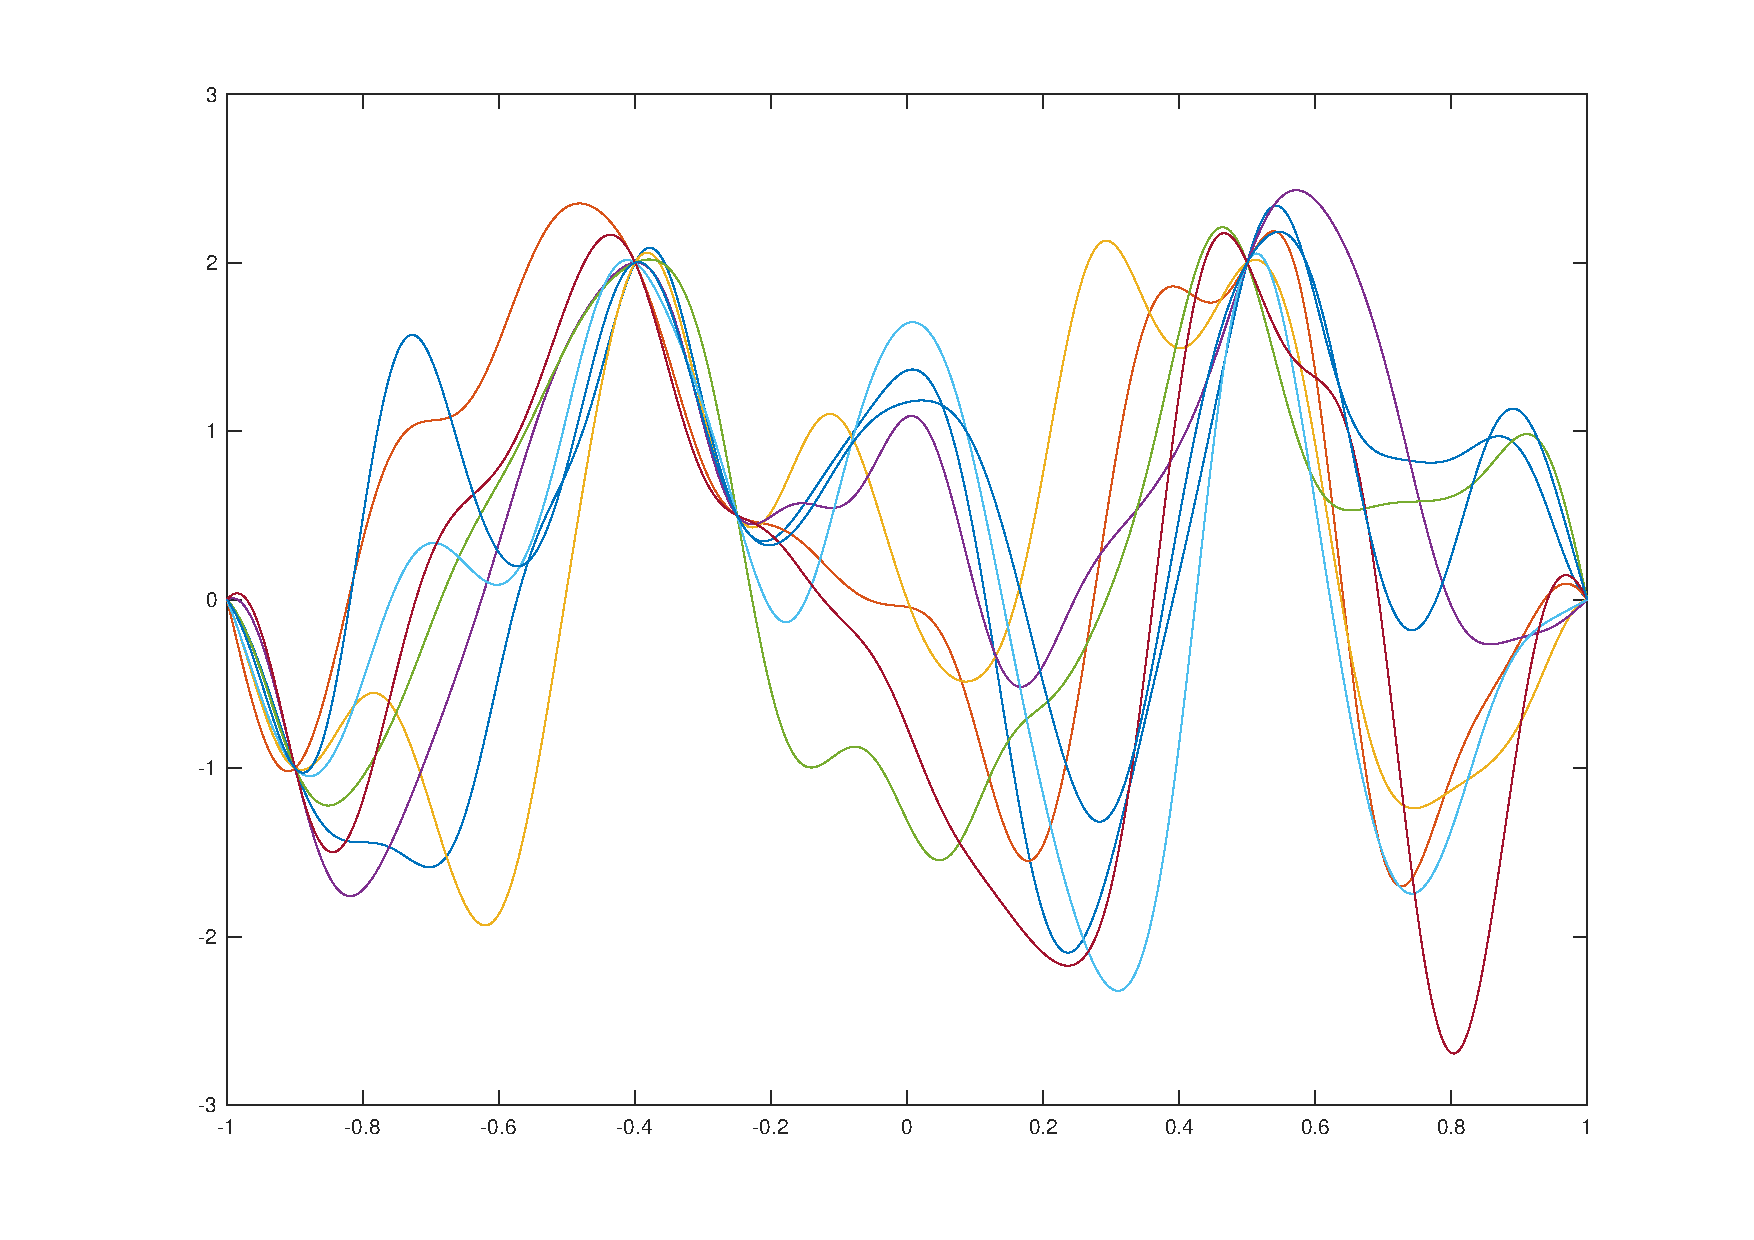
\includegraphics[width=.9\linewidth]{fig/8rnd.pdf}
\caption{The 8 samples drawn from the process specified by the posterior distribution show strong deviations in parts where the variance is high while taking equal values for the points that we specified.}
\label{fig:8rnd}
\end{figure}

\newpage
\begin{lstlisting}[language=Python, caption=python implementation of a gaussian process]
import numpy as np

x1 = np.array([-1, -0.9, -0.4, -0.25, 0.5, 1]);
y1 = np.array([0, -1, 2, 0.5, 2, 0]);

x2 = np.linspace(-1,1,1000);

sigma = 0.3
llambda = 0

def kernel(x,y,sigma,llambda):
    k = np.exp(-(x[:,None] - y[None,:])**2 / (2*sigma**2))
    k = k + np.eye(k.shape[0],k.shape[1]) * llambda
    return k

def gaussian_process(x2,x1,y1,sigma,llambda):
    k11 = kernel(x1,x1,sigma,llambda)
    k12 = kernel(x1,x2,sigma,llambda)
    k22 = kernel(x2,x2,sigma,llambda)

    k11i = np.linalg.inv(k11)
    y2 = k12.T @ k11i @ y1.T
    sig2 = k22 - k12.T @ k11i @ k12
    return y2, sig2

y2,sig2 = gaussian_process(x2,x1,y1,sigma,llambda)
instances8 = np.random.multivariate_normal(y2,sig2,8)
\end{lstlisting}

\begin{lstlisting}[language=Python, caption=python plotting results]
import matplotlib.pyplot as plt
plt.subplot(211)
plt.plot(x1,y1,'o',mfc='None',c='C0',label='data')
plt.plot(x2,y2,'-',c='C0',label='mean prediction')
std2 = 1.96 * np.sqrt(np.diag(sig2))
plt.plot(x2,y2-std2,
	'-.',c='C1',linewidth=0.5,label='95 percentile')
plt.plot(x2,y2+std2,'-.',c='C1',linewidth=0.5)
plt.legend(); plt.title('mean prediction given data')

plt.subplot(212)
plt.plot(instances8.T)
plt.title('random instances drawn from the posterior distribution')

plt.tight_layout()
plt.show()

\end{lstlisting}

\newpage
\nocite{*}
\bibliographystyle{unsrt}
\bibliography{references}

\end{document}

